\documentclass{beamer}
\usepackage[utf8]{inputenc}
\usepackage{algorithm2e}
\usepackage{algorithmic}
\usetheme{Madrid}
\usecolortheme{seahorse}

%used by me%
\usepackage{comment}
\usepackage{xcolor}

\usepackage{multicol}
\usepackage{caption}
\usepackage{graphicx}
\usepackage{ragged2e}
\usepackage{subcaption}
\usepackage{tikz}
\usepackage{pgfplots}

\usepackage[style=apa,backend=bibtex]{biblatex}
\addbibresource{biblio.bib}

\usepackage{appendixnumberbeamer}
\newcommand{\backupbegin}{
   \newcounter{framenumbervorappendix}
   \setcounter{framenumbervorappendix}{\value{framenumber}}
}
\newcommand{\backupend}{
   \addtocounter{framenumbervorappendix}{-\value{framenumber}}
   \addtocounter{framenumber}{\value{framenumbervorappendix}} 
}


% Define custom color
\definecolor{darkskyblue}{RGB}{0, 103, 165}
\definecolor{darkgreen}{RGB}{0,128,0}
\definecolor{amaranth}{rgb}{0.9, 0.17,0.31}
\definecolor{ao-english}{rgb}{0.0,0.5, 0.0}
%used by me%

%\usepackage{enumitem}

%------------------------------------------------------------
%This block of code defines the information to appear in the
%Title page
\title[ENASE'2024] %optional
{An evaluation of the impact of end-to-end query optimization strategies on energy consumption}

%\subtitle{ENACT - ENergy efficiency through ArChitectural Tactics for Software Engineering}

\author[Eros Cede\~no] % (optional)
{\textbf{Eros Cede\~no}\inst{1} \and \underline{Ana Aguilera-Faraco}\inst{2} \and \underline{Denisse Mu\~nante}\inst{3} \and Jorge Correia\inst{1} \and Leonel Guerrero\inst{1} \and and Carlos Sivira\inst{1} \and \underline{Yudith Cardinale}\inst{4}}

% Undergraduate
% Collaboration with other students in the same university and professors in 
\institute[]
{
	\inst{1}
	%Departamento Computación y Tecnología de la Información, 
	Universidad Simón Bolívar, Caracas, Venezuela \and
	\inst{2}%
	%Escuela de Ingeniería Informática, Facultad de Ingeniería, 
	Universidad de Valparaíso, Chile
	\and
	\inst{3}%
	ENSIIE \& SAMOVAR, Évry, France
	\and
	\inst{4}%
	%Centro de Estudios en Ciancia de Datos e IA (ESenCIA), 
	Universidad Internacional de Valencia, Spain
}
\date[April 28-29, 2024]
{The 19th Int. Conf. On Evaluation of Novel \\
Approaches to Software\\
Engineering (ENASE'24)}

\titlegraphic { 
\begin{tikzpicture}[overlay,remember picture]
    \node[left=0.2cm] at (current page.335){
        
\includegraphics[width=1.5cm]{figures/STICAmSud.png}
    };
    \node[right=0.2cm] at (current page.207){
        %
\includegraphics[width=1cm]{figures/logo_ENSIIE.png}
        
\includegraphics[width=2cm]{figures/E4C_logo.png}
    };

\end{tikzpicture}
}

%End of title page configuration block
%------------------------------------------------------------

\begin{document}
%============================================================
\begin{frame}
    \titlepage 
\end{frame}
%============================================================
\begin{frame}{Outline}
        \tableofcontents[hideallsubsections]
\end{frame}

\AtBeginSection[]
{
  \begin{frame}
    \frametitle{Outline}
    \tableofcontents[currentsection,hideallsubsections]
  \end{frame}
}
%============================================================
%============================================================
%\section{Context, Problem and Research objectives}
%\begin{frame}{Context (1/2)}
%\framesubtitle{Green Software}

%\begin{multicols}{2}

%\begin{figure}[h]
%    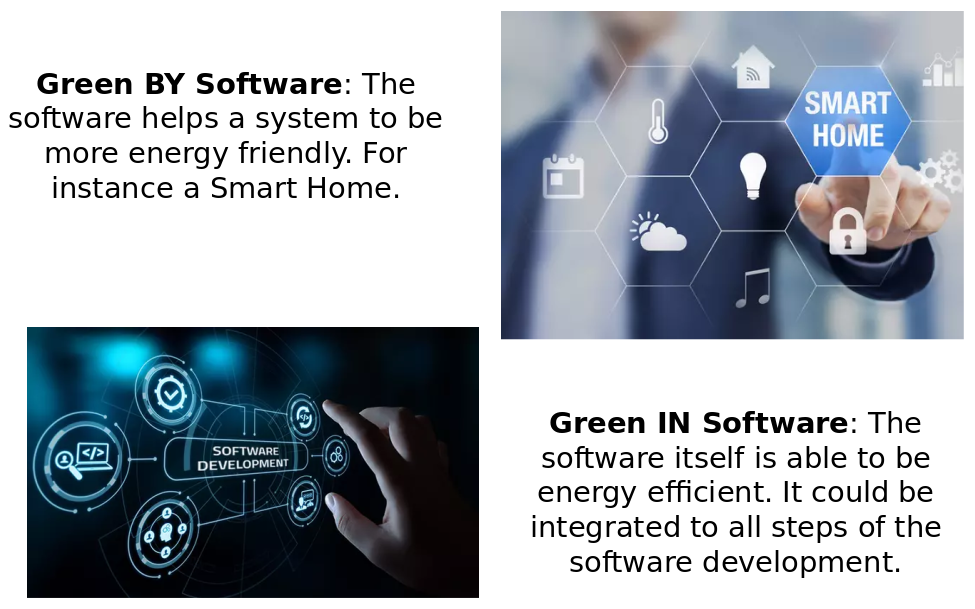
\includegraphics[width=7.7cm]{figures/GreenIT.png}
%%    \caption{Green BY software \textit{vs} Green IN Software}
 %   \centering
%\end{figure}  

%\columnbreak            

%\small{Two new quality attributes:}
% Hacer enfasis que incrementar el conocimiento acerca del consumo energetico ha demostrado que tiene % impacto en el desarrollo de aplicaciones mas energy-friendly
%\begin{itemize}
%\scriptsize
% \item \textbf{Energy awareness:} the level in which stakeholders are aware about the energy consumption that entails the building and usage of software.
% \item \textbf{Energy efficiency:} the level in which a software application is able to spend less energy without affecting its functionalities. 
%\end{itemize}

%\end{multicols}
    
%\end{frame}

\begin{frame}{Context}
\framesubtitle{Evaluation of the energy consumed by Relational Database Systems}

    \begin{itemize}
    \item Software applications intensively receive and transfer data by using a  Relational Database Management Systems (\textit{RDBMS}). 
        \item RDBMS are software components that could require a lot of hardware resources querying larges databases. %This could lead to heavy power  consumption loads on the servers, as well as on the client side.%
% Todas las aplicaciones usan sistemas de bases de datos%
        
        \item Resources are limited and expensive so they must be used wisely. However, developers are not aware of the resource impact they cause when building software. 
    \end{itemize}

\begin{multicols}{2}

\begin{figure}[h]
    
\includegraphics[width=3cm]{figures/energy_cost.png}
    \caption{Energy is expensive}
    \centering
\end{figure}  

\columnbreak            

\begin{figure}[h]
    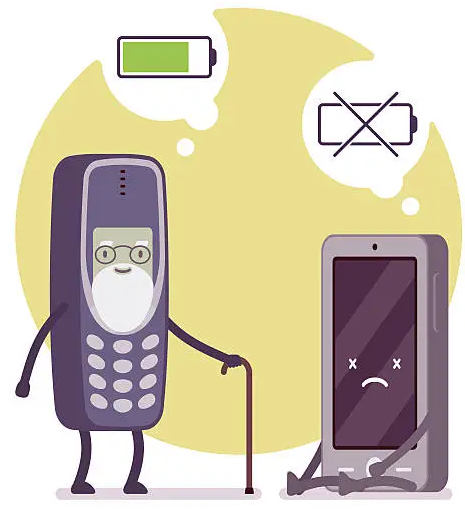
\includegraphics[width=2.5cm]{figures/old_new_phone.png}
    \caption{Applications require more energy every time}
    \centering
\end{figure}  

\end{multicols}
    
\end{frame}

%============================================================
\begin{frame}{Problem and Research objectives}
    \begin{alertblock}{Problem}
        \small{ 
        %Software applications consume more and more energy, but resources are limited.
        Studies are traditionally interested in reducing execution time by implementing databases optimizations strategies such as index or compression. 
        %This could lead to \textbf{heavy energy consumption loads} on the server as well as on the client side. 
        \textbf{However, there are no studies dedicated to analyse the end-to-end (server and client sides) energy impact of these strategies. }}  
        %This could lead to \textbf{heavy energy consumption loads} on the server as well as on the client side.}
    \end{alertblock} 
    
%    \hspace{1cm}
    
    \begin{exampleblock} {Research objectives}
        \small{Our goal is to increase awareness about the \textbf{end-to-end energy impact} of databases optimizations strategies. It can serve as guidelines for supporting developers to choose the strategies that are more energy friendly.
        }
%
%\small{To reach this goal we propose the following RQs:}
         \begin{itemize}
             \scriptsize
             \item RQ1: Does the implementation of database optimization strategies affect the energy consumption of client server applications? 
             \item RQ2: Does the addition of database optimization strategies affect the energy consumption of client server applications?
         \end{itemize}
    \end{exampleblock}
\end{frame}
%============================================================
% Explicar que herramientas tiene cada lado del experimento, Indicar el benchmark utilizado, explicar las 4 configuraciones distintas

\section{Proposal: Evaluating the impact of end-to-end query optimization strategies on energy consumption}

\begin{frame}{Evaluating the impact of end-to-end query optimization strategies on energy consumption}
\framesubtitle{Design of the Study: Setup}

\begin{figure}[b!]
\centering
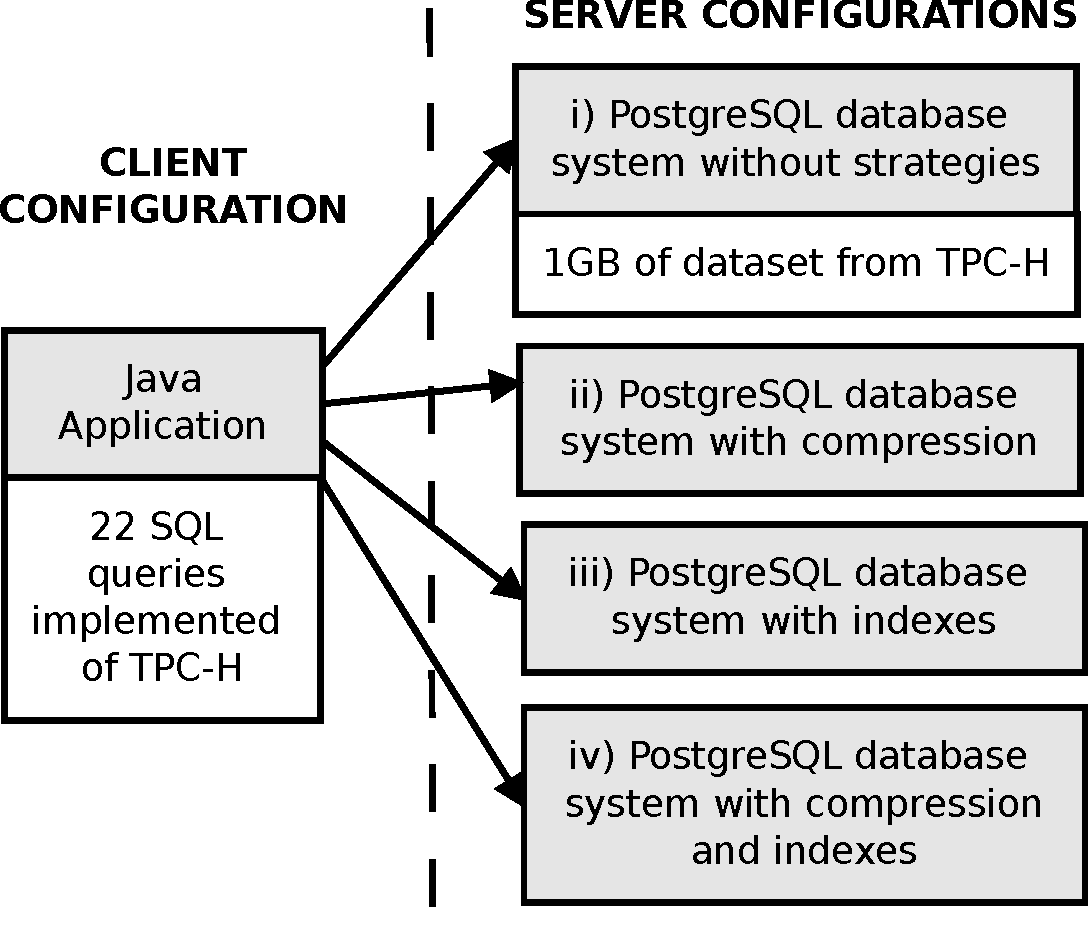
\includegraphics[width=0.5\textwidth]{figures/architecture.pdf}

\label{fig:design}
\end{figure}
\end{frame}

\begin{frame}{Evaluating the impact of end-to-end query optimization strategies on energy consumption}
\framesubtitle{Design of the Study: Algorithm}
\begin{figure}[h]
    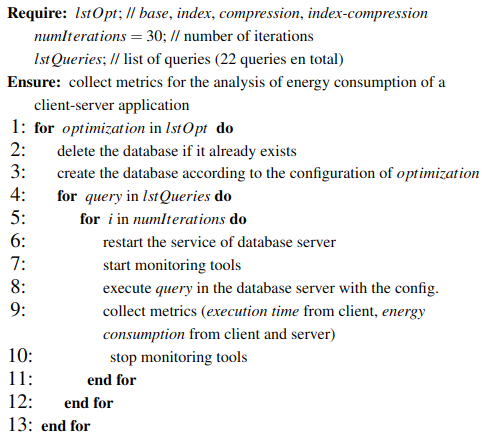
\includegraphics[width=0.5\textwidth]{figures/algorithm.png}
    \centering
\end{figure}  

\end{frame}


\begin{frame}{Evaluating the impact of end-to-end query optimization strategies on energy consumption}
\framesubtitle{\large{\textcolor{blue}{\bf Juliet}}: Minimalist and Energy friendly tool, developed in C++}

% Minimalistic and Energy friendly tool 

\begin{figure}[h]
    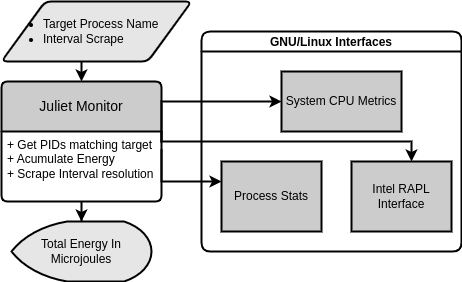
\includegraphics[width=0.6\textwidth]{figures/juliet.drawio (2).png}
    \caption{Juliet Architecture Design}
    \centering
\end{figure}  

\end{frame}

%============================================================
\section{Results of Study}

\small
\begin{frame}{Results of Study}
%\framesubtitle{ and RQ2}

\textbf{RQ1:} Does the implementation of database optimization strategies affect the energy consumption of client server applications?\\
\textbf{RQ2:} Does the addition of database optimization strategies affect the energy consumption of client server applications?

\scriptsize
\begin{table}[]
\caption{\scriptsize{Sample Query Results. \textbf{AEC}: Average of energy consumption. \textbf{RSEC}: Relative standard deviation. \textbf{DEC:} Difference of EC vs Base }}
\begin{tabular}{|lllllll|}
\hline
\multicolumn{7}{|c|}{Query 22}                                                     \\ \hline
\multicolumn{1}{|l|}{}   & \multicolumn{3}{c|}{Client}                                                          & \multicolumn{3}{c|}{Server}                                      \\ \hline
\multicolumn{1}{|l|}{}   & \multicolumn{1}{l|}{AEC}    & \multicolumn{1}{l|}{RSEC} & \multicolumn{1}{l|}{\%DEC}   & \multicolumn{1}{l|}{AEC}     & \multicolumn{1}{l|}{RSEC} & \%DEC   \\ \hline
\multicolumn{1}{|l|}{Base}  & \multicolumn{1}{l|}{119.39} & \multicolumn{1}{l|}{0.06} & \multicolumn{1}{l|}{-}     & \multicolumn{1}{l|}{4427.2}  & \multicolumn{1}{l|}{0.07} & -     \\ \hline
\multicolumn{1}{|l|}{Index}  & \multicolumn{1}{l|}{16.22}  & \multicolumn{1}{l|}{0.07} & \multicolumn{1}{l|}{\textbf{86.41}} & \multicolumn{1}{l|}{1.41}    & \multicolumn{1}{l|}{0.19} & \textbf{99.97} \\ \hline
\multicolumn{1}{|l|}{Compression}  & \multicolumn{1}{l|}{118.93} & \multicolumn{1}{l|}{0.06} & \multicolumn{1}{l|}{-}     & \multicolumn{1}{l|}{4387.18} & \multicolumn{1}{l|}{0.07} & -     \\ \hline
\multicolumn{1}{|l|}{Index-Compression} & \multicolumn{1}{l|}{16.26}  & \multicolumn{1}{l|}{0.05} & \multicolumn{1}{l|}{\textbf{86.38}} & \multicolumn{1}{l|}{1.2}     & \multicolumn{1}{l|}{0.19} & \textbf{99.97} \\ \hline
\end{tabular}

\end{table}
\end{frame}
%=====================================================
\small
\begin{frame}{Results of Study}
%\framesubtitle{ and RQ2}

\textbf{RQ1:} Does the implementation of database optimization strategies affect the energy consumption of client server applications?\\
\textbf{RQ2:} Does the addition of database optimization strategies affect the energy consumption of client server applications?

\scriptsize
\begin{table}[]
\caption{\scriptsize{Sample Query Results. \textbf{AEC}: Average of energy consumption. \textbf{RSEC}: Relative standard deviation. \textbf{DEC:} Difference of EC vs Base }}
\begin{tabular}{|lllllll|}
\hline
\multicolumn{7}{|c|}{Query 17}                                                     \\ \hline
\multicolumn{1}{|l|}{}   & \multicolumn{3}{c|}{Client}                                                          & \multicolumn{3}{c|}{Server}                                      \\ \hline
\multicolumn{1}{|l|}{}   & \multicolumn{1}{l|}{AEC}    & \multicolumn{1}{l|}{RSEC} & \multicolumn{1}{l|}{\%DEC}   & \multicolumn{1}{l|}{AEC}     & \multicolumn{1}{l|}{RSEC} & \%DEC   \\ \hline
\multicolumn{1}{|l|}{Base}  & \multicolumn{1}{l|}{43.78} & \multicolumn{1}{l|}{0.08} & \multicolumn{1}{l|}{-}     & \multicolumn{1}{l|}{393.82}  & \multicolumn{1}{l|}{0.03} & -     \\ \hline
\multicolumn{1}{|l|}{Index}  & \multicolumn{1}{l|}{22.74}  & \multicolumn{1}{l|}{0.09} & \multicolumn{1}{l|}{\textbf{48.06}} & \multicolumn{1}{l|}{241.73}    & \multicolumn{1}{l|}{0.01} & \textbf{38.62} \\ \hline
\multicolumn{1}{|l|}{Compression}  & \multicolumn{1}{l|}{23.76} & \multicolumn{1}{l|}{0.08} & \multicolumn{1}{l|}{\textbf{45.73}}     & \multicolumn{1}{l|}{265.73} & \multicolumn{1}{l|}{0.02} & \textbf{32.53}     \\ \hline
\multicolumn{1}{|l|}{Index-Compression} & \multicolumn{1}{l|}{23.39}  & \multicolumn{1}{l|}{0.10} & \multicolumn{1}{l|}{\textbf{46.56}} & \multicolumn{1}{l|}{238.51}     & \multicolumn{1}{l|}{0.02} & \textbf{39.44} \\ \hline
\end{tabular}

\end{table}
\end{frame}
%============================================================

\begin{frame}{Results of Study}

\framesubtitle{RQ1 and RQ2}
%=========
% 16 de las 22 queries tienen comportamiento adecuado,
%=========
\begin{multicols}{2}

\centerline{\textbf{RQ1}}
\begin{itemize}
    \item \small{The \textbf{index} strategy reduce between [1.15, 103.17] J for the client side energy consumption, whilst for the \textbf{compression} was [1.28, 20.02] J.}
    \item \small{ For the server side, the \textbf{index} strategy reduce between [1.66, 4425.79] J, whilst the \textbf{compression} reduced between [1.21, 128.08] J.}
\end{itemize}

\centerline{\textbf{Conclusion: I $>$ C}}

\columnbreak
\centerline{\textbf{RQ2}}

\begin{itemize}
\item \small{ For the \textbf{index-compression} strategy the reduction
of the energy consumption was between [0.92, 86.38] J for the client
side, whilst for the server side was between [1.33, 4426] J. These values are similar to the values obtained for the \textbf{index} strategy.}
\end{itemize}
\centerline{\textbf{Conclusion: I + C $\equiv$ I}}
\end{multicols}

\end{frame}

%============================================================
% Nombrar las 3 queries que generan incremento y mencionar las otras 3 que no hacen cambio, mencionar que no se ve nada diferente en estas queries y que es necesario un estudio posterior
\begin{frame}{Results of Study}
\framesubtitle{Some Exceptions: ....}

\scriptsize
\begin{table}[]
\begin{tabular}{|lllllll|}
\hline
\multicolumn{7}{|c|}{Query 05}                                                                                                                                                 \\ \hline
\multicolumn{1}{|l|}{}   & \multicolumn{3}{c|}{Client}                                                       & \multicolumn{3}{c|}{Server}                                     \\ \hline
\multicolumn{1}{|l|}{}   & \multicolumn{1}{l|}{AEC}   & \multicolumn{1}{l|}{RSEC} & \multicolumn{1}{l|}{\%DEC} & \multicolumn{1}{l|}{AEC}   & \multicolumn{1}{l|}{RSEC} & \%DEC    \\ \hline
\multicolumn{1}{|l|}{Base}  & \multicolumn{1}{l|}{18.78} & \multicolumn{1}{l|}{0.13} & \multicolumn{1}{l|}{-}   & \multicolumn{1}{l|}{21.43} & \multicolumn{1}{l|}{0.06} & -      \\ \hline
\multicolumn{1}{|l|}{Index}  & \multicolumn{1}{l|}{18.32} & \multicolumn{1}{l|}{0.11} & \multicolumn{1}{l|}{-}   & \multicolumn{1}{l|}{26.50} & \multicolumn{1}{l|}{0.07} & \textbf{-23.68} \\ \hline
\multicolumn{1}{|l|}{Compression}  & \multicolumn{1}{l|}{18.12} & \multicolumn{1}{l|}{0.12} & \multicolumn{1}{l|}{-}   & \multicolumn{1}{l|}{18.18} & \multicolumn{1}{l|}{0.1}  & 15.13  \\ \hline
\multicolumn{1}{|l|}{Index-Compression} & \multicolumn{1}{l|}{19.14} & \multicolumn{1}{l|}{0.11} & \multicolumn{1}{l|}{-}   & \multicolumn{1}{l|}{25.04} & \multicolumn{1}{l|}{0.08} & \textbf{-16.84} \\ \hline
\end{tabular}
\end{table}


\scriptsize{
\begin{algorithmic}[1]
\textbf{SELECT}  n\_name,
	\textbf{sum(}l\_extendedprice * (1 - l\_discount)\textbf{)} \textbf{as} revenue \linebreak
\textbf{FROM} customer, orders,	lineitem,	supplier, nation,
	region\linebreak
\textbf{WHERE}
	c\_custkey = o\_custkey\linebreak
	\textbf{AND} l\_orderkey = o\_orderkey\linebreak
	\textbf{AND} l\_suppkey = s\_suppkey\linebreak
	\textbf{AND} c\_nationkey = s\_nationkey\linebreak
	\textbf{AND} s\_nationkey = n\_nationkey\linebreak
	\textbf{AND} n\_regionkey = r\_regionkey\linebreak
	\textbf{AND} r\_name = 'ASIA'\linebreak
	\textbf{AND} o\_orderdate \geq date\  '1993-01-01'\linebreak
	\textbf{AND} o\_orderdate < date\ '1993-01-01' + interval\ '1'\ year\linebreak
\textbf{GROUP BY}\ n\_name\linebreak
\textbf{ORDER BY}\ revenue\ \textbf{DESC}\linebreak
\textbf{LIMIT 1};
\end{algorithmic}
}

\end{frame}
%============================================================
\section{Threats to validity, Conclusion and Future work}
\begin{frame}{Threats to validity, Conclusion and Future work (1/2)}

\begin{block} {Threats to validity}
         \begin{itemize}
             \small
             \item \textbf{Internal validity:} Juliet could introduce bias.
             \item \textbf{Construct validity:} Same computer used for running the client and server.
             \item \textbf{External validity:} Benchmarking limited to 22 specific queries, our results cannot be generalized.
         \end{itemize}
\end{block}

\begin{exampleblock} {Conclusion}
         \begin{itemize}
             \small
             \item \textbf{Indexation tends to be more effective than data compression to reduce the energy} consumed by the execution of the majority of the queries (16/22 queries). The addition of indexation and compression does not lead to a better result comparing with indexation.
             \item \textbf{More experiments are needed to understand the reason of why some queries do not follow this tendency:} i) 3/22 queries increase energy consumption, and ii) 3/22 queries do not show any effect.  

         \end{itemize}
\end{exampleblock}

\end{frame}
%============================================================
\begin{frame}{Threats to validity, Conclusion and Future work (2/2)}

\begin{block} {Future work}
         \begin{itemize}
             \small
             \item Run new experiments in a real distributed software architecture.
             %Improve the scenario of the experiments running client and server in different machines.
             \item Run new experiments
             %Apply the same empirical evaluation 
             over other RDBMS and NoSQL datasets.
             \item Classify the queries according their complexity, responses time and size to run new experiments.
             \item Consider the trade-off of energy consumption of database optimization strategies with other resources such as CPU, I/O usage, and memory. 
             \item Run new experiments to compare Juliet with other tools like Scaphandre or PowerAPI. 
         \end{itemize}
\end{block}

\end{frame}

%============================================================
\begin{frame}
\frametitle{}

\begin{huge}
\begin{center}

\textbf{\textcolor{ao-english}{Thank you!}}
\end{center}
\end{huge}

\begin{center}
\textbf{16-10216@usb.ve}

\hspace{2.5cm}

\scriptsize{\textcolor{ao-english}{This work has been partially supported by the \textbf{STIC AmSud project}: ``GreenSE4IoT - Towards Energy-efficient Software for Distributed Systems'' [STIC-AMSUD 22-STIC-04], \\
and has been partially carried out at the \textbf{Energy4Climate Interdisciplinary Center (E4C)} of IP Paris and École des Ponts ParisTech, which is in part supported by 3rd Programme d’Investissements d’Avenir [ANR-18-EUR-0006-02].}}
%Finally, thanks to \textbf{ENSIIE} school engineer for funding my registration to ENASE'24.}
%}
\end{center}

\titlegraphic { 
\begin{tikzpicture}[overlay,remember picture]
    \node[left=0.2cm] at (current page.335){
        
\includegraphics[width=1.5cm]{figures/STICAmSud.png}
    };
    \node[right=0.2cm] at (current page.207){
        
\includegraphics[width=1cm]{figures/logo_ENSIIE.png}
        
\includegraphics[width=2cm]{figures/E4C_logo.png}
    };

\end{tikzpicture}
}

\begin{multicols}{3}

\begin{figure}
    \centering
    
\includegraphics[scale=0.25]{figures/STICAmSud.png}
\end{figure}

\columnbreak            

\begin{figure}
    \centering
    
\includegraphics[scale=0.25]{figures/E4C_logo.png}
\end{figure}

%\columnbreak            

%\begin{figure}
%    \centering
%    
\includegraphics[scale=0.3]{figures/logo_ENSIIE.png}
%\end{figure}

\end{multicols}


\end{frame}

%Motivacion corta y concisa%

%Explicar que este trabajo es reelevante porque permite analizar tanto cliente como servidor%

%Slide con las limitations%

% Threads to validity%

% Para las Research questions 2 contraejemplos por resultado obtenido indicando porcentajes%

%Juliet en el diseno%

%Grafica para Juliet en cuanto al metodo de recoleccion de informacion de energia%


%Justificar por que la compresion aumenta el consumo energetico (EN EL SLIDE)%
%Agradecimientos a los proyectos que apoyaron%

%Maximo 15 diapositivas%

%Enfasis en lo principal%

\end{document}

